\documentclass[a4paper, 11pt]{article}
\usepackage{graphicx, float, url, hyperref, lscape, afterpage, amsthm, amsmath}
%\usepackage[margin=1in]{geometry}
\title{Numerical Integration: Planck's Theory of Blackbody Radiation}
\author{CS 236 MP2\\ Joshua Frankie Rayo\\ 2011-19612\\ Scientific Computing Laboratory}
\date{\today}
\newtheorem{definition}{Definition}

\begin{document}
\maketitle

\tableofcontents
\listoffigures
\listoftables

\section{Problem Description}
The problem can be found in Computer Problem 8.11 - Scientific Computing (An Introductory Survey) 2e Michael Heath. \cite{bib:sci}

Planck's theory of blackbody radiation leads to the integral
\begin{equation}\label{eqn:planck}
I(x) = \int_0^{\infty} \frac{x^3}{e^x-1}\;dx
\end{equation}

Evaluate this integral using each of the methods and compare their efficiency and accuracy.
\begin{itemize}
	\item Composite Simpson's Rule
	\item Adaptive Quadrature (bounded and unbounded)
	\item Gauss Laguerre Quadrature
\end{itemize}

\section{Preliminaries}
\subsection{Planck's Law of Blackbody Radiation}
Planck's Law suggests that the radiated energy of a medium due to absorbed radiation frequency at a constant temperature is given by

\begin{equation*}
E(v) = \frac{8\pi}{c^3} \ \frac{\hbar v^3}{e^{\frac{\hbar v}{kT}}-1}
\end{equation*}

where $k$ is the Boltzmann constant, $\hbar$ the Planck constant, $c$ the speed of light in the medium and $T$ its absolute temperature. In classical physics, radiated energy is proportional to the square of frequency that leads to a phenomenon called 'ultraviolet catastrophe'.

\subsection{Polylogarithms}
For a complex number $x$ of modulus $|x|<1$, the polylogarithm of order $n$ evaluated at $x$ denoted $P_x(x)$ is defined by:

\begin{equation}\label{eqn:poly}
P_n(x) = \sum_{k=1}^{\infty} \frac{x^k}{k^n}
\end{equation}

Some values of polylogarithms include:

\begin{align*}
P_1(x) &= -\ln(1-x)\\
P_0(x) &= \frac{-x}{x-1}\\
P_{-1}(x) &= \frac{x}{(x-1)^2}\\
P_{-2}(x) &= \frac{-x(x+1)}{(x-1)^3}\\
P_{-3}(x) &= \frac{x(x^2+4x+1)}{(x-1)^4}
\end{align*}

For $n \leq 1, n \in \mathbf{Z}$ , the value of $P_n(x)$ converges.

\subsection{Gaussian Quadrature}
The Gaussian Quadrature\cite{bib:sci} is targeted to approximate an integral by taking the weighted sum of integrand values sampled at special points (called abscissas). The abscissas and weights are calculated in a special way so that the rule provides a precise answer for all polynomials up to certain degree. 

\begin{equation}
\int_{a}^{b}\omega(x)f(x)\;dx \approx \sum_{i=1}^{n} w_i f(x_i)
\end{equation}

\subsection{Laguerre Polynomials}
The Laguerre polynomials\cite{bib:lagpoly} $\lbrace L_n(x)\rbrace$ are solutions to the associated Laguerre differential equation
\begin{equation}\label{eqn:lpoly}
xy''+(1-x)y'+ny=0
\end{equation}
They are given by the sum
\begin{equation}
y=L_n(x) = \sum_{i=0}^{n}\frac{(-1)^i}{i!}
\begin{pmatrix}
n\\k
\end{pmatrix}
(x)^k
\end{equation}
Where $n$ is the degree of a particular Laguerre polynomial. This is only a special case of the generalized Laguerre polynomials $L^k_n(x)$. The first few Laguerre polynomials are given below.

\begin{align*}
L_0(x) &= 1 \\
L_1(x) &= -x+1 \\
L_2(x) &= \frac{1}{2} \left(x^2-4x+2\right) \\
L_3(x) &= \frac{1}{6} \left(-x^3+9x^2-18x+6\right) \\
L_4(x) &= \frac{1}{24} \left(x^4-16x^3+72x^2-96x+24\right) \\
L_5(x) &= \frac{1}{120} \left(-x^5+25x^4-200x^3+600x^2-600x+120\right) \\
L_6(x) &= \frac{1}{720} \left(x^6-36x^5+450x^4-2400x^3+5400x^2-4320x+720\right) \\
L_7(x) &=  \frac{1}{5040} \\ &\left(-x^7+49x^6-882x^5+7350x^4-29400x^3+529200x^2-35280x+5040\right) \\
L_8(x) &=  \frac{1}{40320} \\ &(x^8-64x^7+1568x^6-18816x^5+117600x^4-376320x^3+564480x^2 \\
&-322560x+40320) \\
L_9(x) &=  \frac{1}{362880}(- x^9 + 81x^8 - 2592x^7 + 42336x^6 - 381024x^5 + 1905120x^4 - \\ & 5080320x^3 + 6531840x^2 - 3265920x + 362880) \\
L_{10}(x) &= \frac{1}{3628800}(x^{10} - 100x^9 + 4050x^8 - 86400x^7 + 1058400x^6 - 7620480x^5 \\ & + 31752000x^4 - 72576000x^3 + 81648000x^2 - 36288000x + 3628800)
\end{align*}

\begin{figure}[H]
	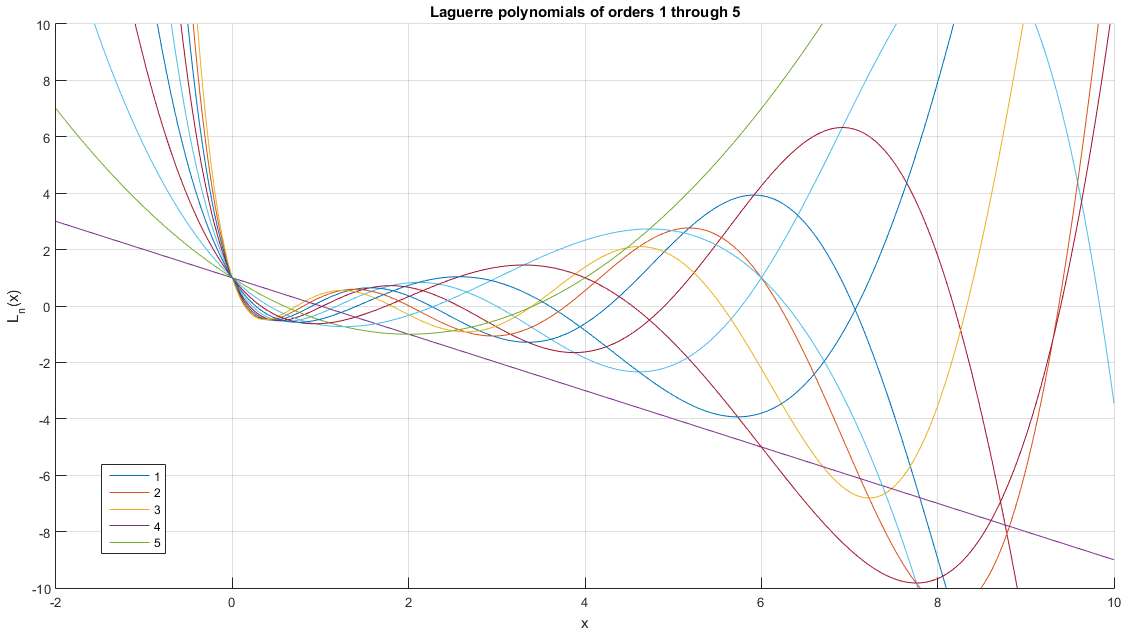
\includegraphics[width=\textwidth]{laguerre}
	\caption{Graph of Laguerre polynomials or orders 1 to 5}
\end{figure}

For nonnegative integer values of $n$, the polynomials are orthogonal over $[0, \infty)$ with respect to the weighting function $e^{-x}$,

\begin{align}
\int_{0}^{\infty}e^{-x}L_n(x)L_m(x)\;dx &= \frac{(n+k)!}{n!}\delta(m,n) \\
\delta(m,n) &=
\begin{cases}
0, m \neq n \\
1, m = n
\end{cases}
\end{align}

where $\delta(m,n)$ is the Kronecker delta function. Furthermore, they satisfy the recurrence relations
\begin{align*}
(n+1)L_{n+1}(x) &= (2n+1-x)L_n(x) - nL_{n-1}(x) \\
xL'_{n}(x) &= nL_n(x) - nL_{n-1}(x)
\end{align*}

For the generalized cases mentioned above, one can read \cite{bib:assoc}, \cite{bib:lagdiff} and \cite{bib:delta}.

\subsection{Gauss-Laguerre Quadrature}
The Generalized Gauss-Laguerre quadrature \cite{bib:laguerre}, is a Gaussian quadrature over the interval $[a, \infty)$ with weighting function $W(x) = x^a e^{-x}$. This weighting function is only a specific case of the generalized weighting function. In this paper, $a=0$. The $n$ nodal abscissas and their corresponding weights are characterized by
\begin{align}\label{eqn:glint}
L_n(x_i) &= 0 \\
w_i &= \frac{x_i}{(n+1)^2\lbrack L_{n+1}(x_i) \rbrack^2} \\
i &= 1, 2, \ldots n
\end{align}

The derivation of equation (9) can be found in \cite{bib:laguerre} that uses the properties of orthogonal functions and factorial notation. The relationship described in equation (10) follows from the property that $L_n(x)$ has $n$ real roots, which its proof shall not be explained here. Nodal abscissas and weights from order 0 to 10 are listed below.

\begin{table}[H]
	\centering
	\begin{tabular}{c | c c}
		$n$ & $x_i$ & $w_i$ \\
		\hline
		0 & - & - \\
		\hline
		1 & 1 & 1 \\
		\hline
		2 & 0.585786437626905 & 0.853553390593274 \\
		  & 3.414213562373095 & 0.146446609406726 \\
		\hline
		3 & 0.415774556783479 & 0.711093009929174 \\
		  & 2.294280360279045 & 0.278517733569238 \\
		  & 6.289945082937476 & 0.010389256501586 \\
		\hline
		4 & 0.322547689619392 &  0.603154104341638 \\
		& 1.745761101158349 &  0.357418692437795\\
		& 4.536620296921130 &  0.038887908515005\\
		& 9.395070912301121 &  0.000539294705561\\
		\hline
		5 & 0.263560319718141 &  0.521755610582809\\
		& 1.413403059106519 &  0.398666811083170\\
		& 3.596425771040735 &  0.075942449681705\\
		& 7.085810005858809 &  0.003611758679922\\
		& 12.640800844275811 &  0.000023369972386\\
		\hline
		6 & 0.222846604179261 &  0.458964673949961\\
		& 1.188932101672622 &  0.417000830772124\\
		& 2.992736326059316 &  0.113373382074044\\
		& 5.775143569104473 &  0.010399197453150\\
		& 9.837467418382694 &  0.000261017202815\\
		& 15.982873980601580 &  0.000000898547906\\
	\end{tabular}
\end{table}

\begin{table}[H]
	\centering
	\begin{tabular}{c | c c}
		7 & 0.193043676560362 &  0.409318951701294\\
		& 1.026664895339196 &  0.421831277861697\\
		& 2.567876744950756 &  0.147126348657497\\
		& 4.900353084526437 &  0.020633514468720\\
		& 8.182153444562976 &  0.001074010143281\\
		& 12.734180291797712 &  0.000015865464349\\
		& 19.395727862262582 &  0.000000031703155\\
		\hline
		8 & 0.170279632305101 &  0.369188589341639\\
		& 0.903701776799376 &  0.418786780814370\\
		& 2.251086629866124 &  0.175794986637181\\
		& 4.266700170287834 &  0.033343492261192\\
		& 7.045905402392907 &  0.002794536235229\\
		& 10.758516010181676 &  0.000090765087733\\
		& 15.740678641277766 &  0.000000848574672\\
		& 22.863131736889201 &  0.000000001048001\\
		\hline
		9 & 0.152322227731808 &  0.336126421797967 \\
		& 0.807220022742257 &  0.411213980423970\\
		& 2.005135155619310 &  0.199287525370956\\
		& 3.783473973331470 &  0.047460562765595\\
		& 6.204956777876078 &  0.005599626610804\\
		& 9.372985251687959 &  0.000305249767093\\
		& 13.466236911092070 &  0.000006592123026\\
		& 18.833597788991732 &  0.000000041107693\\
		& 26.374071890927347 &  0.000000000032909\\
		\hline
		10 & 0.137793470540493 &  0.308441115765012\\
		& 0.729454549503174 &  0.401119929155235\\
		& 1.808342901740227 &  0.218068287612036\\
		& 3.401433697855499 &  0.062087456098448\\
		& 5.552496140061514 &  0.009501516975263\\
		& 8.330152746770436 &  0.000753008388576\\
		& 11.843785837890040 &  0.000028259233496\\
		& 16.279257831388321 &  0.000000424931398\\
		& 21.996585811974988 &  0.000000001839565\\
		& 29.920697012275156 &  0.000000000000991\\
	\end{tabular}
\end{table}

After getting the nodal abscissas $x_i$ and corresponding nodal weights $w_i$, the integral can be approximated as a linear combination of nodal weights and value of the integrand at each nodal abscissas.

\begin{align}
\int_{0}^{\infty}f(x)\;dx &= \int_{0}^{\infty}e^{-x}\;\lbrack e^xf(x) \rbrack\;dx \\
&\approx \sum_{i=1}^{n}w_i\;\lbrack e^{x_i}f(x_i) \rbrack
\end{align}

\section{Analytical Solution}
Note that the integral in \ref{eqn:int} cannot be evaluated in such a closed form. A possible analytical solution of equation (\ref{eqn:planck}) suggested by MATLAB is characterized by:

\begin{equation}\label{eqn:int}
	I(x) = \left( x^3 \ln(1-e^x) - 6x \, \mathnormal{P}_3(e^x) + 6 \, \mathnormal{P}_4(e^x) + 3x^2 \, \mathnormal{P}_2(e^x) - \frac{x^4}{4} \right) _0 ^ {\infty}
\end{equation}

Where $P_n(x)$ is the polylogarithm of order $n$ evaluated at $x$. After solving equation (\ref{eqn:int}) using (\ref{eqn:poly}), the integral turns out to be:
\begin{equation}
I(x) = \int_0^{\infty} \frac{x^3}{e^x-1} \ dx = \frac{\pi^4}{15} = 6.493939402266829\ldots
\end{equation}

\section{Methodology}
\subsection{Machine Specifications}
Succeeding computations are done in MATLAB R2015a 64-bit using 64-bit Windows 7 operating system with Intel\textregistered \hfil Core\texttrademark \hfil i3-2310M CPU with 4 logical processors and 8.00GB of RAM.

\subsection{Analysis of Integrand}
We let $F(x) = \frac{x^3}{e^x-1}$. With direct evaluation, $F(0)=\infty$ and $F(\infty)=0$. 

However, note that $\lim_{x \rightarrow 0^+} F(x) = 0$ and $\lim_{x \rightarrow \infty} F(x) = 0$ as described by the graph below:

\begin{figure}[H]
	\centering
	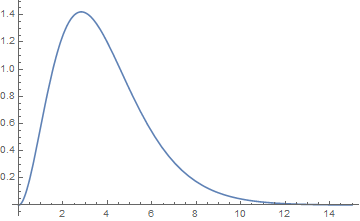
\includegraphics[width=0.85\textwidth]{graph}
	\caption{Graph of $F(x)$, $x \in [0, 15]$}
\end{figure}

One cannot evaluate directly $F(0)$. But for the purpose of integration, it is reasonable to say that $$F(0) = \lim_{x \rightarrow 0^+} F(x) = 0$$

\subsection{Composite Simpson's 2/3 Rule}
Let $h=0.001$ and truncate the interval of integration at selected end points. Next,  accuracy and the running time of each selected interval is compared.

\begin{table}[H]
	\begin{tabular}{c | c | c c}
		Interval & $\tilde{I}(x)$ & Running Time & Absolute Error \\
		\hline
		$[0, 20]$ & 6.493920179948209 & 0.122800 s & 1.922231861861690e-05 \\
		$[0, 40]$ & 6.493939402266595 & 0.266601 s & 2.327027459614328e-13 \\
		$[0, 100]$ & 6.493939402266595 & 0.543443 s & 2.327027459614328e-13 \\
	\end{tabular}
	\caption{Interval truncation analysis of numerical integration using Simpson's rule}
\end{table}

The truncated interval [0, 40] already gives a very good approximation to the real value, given that $h=0.001$.

\subsection{Adaptive Quadrature}\label{sec:adapt}
The quadrature rules used for approximation are the trapezoid and Simpson's rules to gain optimal convergence rate. Rough estimate of the integral is set to 6. We compare again the accuracy and the running time of each selected interval.

\begin{table}[H]
	\begin{tabular}{c | c | c c}
		Interval & $\tilde{I}(x)$ & Running Time & Absolute Error \\
		\hline
		$[0, 20]$ & 6.493914876742610 & 0.397 s & 2.452552421861043e-5 \\
		$[0, 40]$ & 6.493934100801498 & 0.497 s & 5.301465330731503e-6 \\
		$[0, 100]$ & 6.493934082444151 & 0.422 s & 5.319822677485320e-6 \\
	\end{tabular}
	\caption{Interval truncation analysis of numerical integration using adaptive quadrature rule}
\end{table}

On the third chosen interval, the absolute error is unexpectedly bigger than the second one. It suggests that further truncation is not necessary. In terms of accuracy and efficiency, composite Simpson's rule demonstrated earlier is better than adaptive quadrature.

\subsection{Gauss-Laguerre Quadrature}
Using equation \ref{eqn:glint}, the integral in equation \ref{eqn:planck} can be approximated by:

\begin{align}
I(x) &= \int_0^{\infty} \frac{x^3}{e^x-1}\;dx \\
&\approx \sum_{i=1}^{n} w_i \left( \frac{e^{x_i}\;x_i^3}{e^{x_i}-1} \right)
\end{align}

The table below illustrates the comparison between the accuracy and running time employing Gauss-Laguerre quadrature rule of orders 1 to 10.
\begin{table}[H]
	\centering
	\begin{tabular}{c | c | c c}
		$n$ & $\tilde{I}(x)$ & Running Time & Absolute Error \\
		\hline
		$1$ & 1.581976706869326 & 0.102988948626483 s & 4.911962695397502 \\
		$2$ & 6.413727469517580 & 0.129845452799399 s & 0.080211932749248 \\
		$3$ & 6.481130171540009 & 0.165626431026537 s & 0.012809230726819 \\
		$4$ & 6.494535639802607 & 0.179893078339982 s & 5.962375357793093e-04 \\
		$5$ & 6.494313365790788 & 0.200711475238384 s & 3.739635239599082e-04 \\
		$6$ & 6.493941414321306 & 0.225141007276518 s & 2.012054477695813e-06 \\
		$7$ & 6.493918910309293 & 0.249080844171870 s & 2.049195753528466e-05 \\
		$8$ & 6.493935665352286 & 0.279867616147429 s & 3.736914542251668e-06 \\
		$9$ & 6.493940204074303 & 0.301929310893371 s & 8.018074746374282e-07 \\
		$10$ & 6.493939967652644 & 0.330046218033586 s & 5.653858154985869e-07 \\
	\end{tabular}
	\caption{Performance analysis of Gauss-Laguerre quadrature at different orders}
\end{table}

Notice the inconsistency of absolute errors of orders 6, 7 and 8.

\subsection{Adaptive Quadrature Rule for Improper Integrals}
There are two ways of solving improper integrals of the form
\begin{equation}
F(x) = \int_{0}^{\infty} f(x) \ dx
\end{equation}
We integrate $f(x)$ from 0 to a finite value $b$, then let $b$ approach $\infty$:
\begin{equation}
F(x) = \lim_{b \rightarrow \infty} \int_{0}^{b} f(x) \ dt
\end{equation}
If the limit of right hand side exists, then we are done. This approach is already illustrated in section \ref{sec:adapt} where the integral is approximated using adaptive quadrature rule in some finite interval then let the interval get large.


Another way is to transform this to an integral with bounded limits
\begin{align}\label{eqn:spec}
\int_{0}^{\infty} f(x) \ dx = \int_{u=g(0)}^{u=g(\infty)} f(u) \ du, \ u=g(x) \\ \ g(0) < g(\infty) < \infty
\end{align}
by introducing change of variable.

This approach is motivated by the substitution rule:

\begin{equation}
\int_{x=0}^{x=\infty} f(g(x))g'(x) \ dx = \int_{u=g(0)}^{u=g(\infty)} f(u) \ du \ , \ u=g(x)
\end{equation}

The objective is to transform the limits of integration in \ref{eqn:planck} from  $[0,\infty]$ to $[0, 1]$. With the constraints illustrated in equation \ref{eqn:spec}, we should choose a strictly increasing function $g: [0, \infty] \rightarrow [0, 1]$ such that $0=g(0)<g(\infty)<\infty.$ A possible substitution is to let
\begin{equation}\label{eqn:subs}
u = g(x) = \frac{x}{x+1}
\end{equation}
This gives $g(0)=0$ and $g(\infty)=\lim_{x \rightarrow \infty}g(x)=1$ by L'Hopital's rule. From equation \ref{eqn:subs}, we have
\begin{equation}\label{eqn:xofu}
x = \frac{u}{1-u} \ , \ dx=(1+x)^2\;du=\frac{du}{(1-u)^2}
\end{equation}
Using equations \ref{eqn:spec} and \ref{eqn:xofu}, the transformation is illustrated by
\begin{equation}\label{eqn:trans}
\int_0^{\infty}f(x)\;dx = \int_{0}^{1} f\left(\frac{u}{1-u}\right)\;\frac{du}{(1-u)^2}
\end{equation}

Using equation \ref{eqn:trans}, the original problem \ref{eqn:planck} can now be transformed to
\begin{equation}
I(x) = \int_0^{\infty} \frac{x^3}{e^x-1}\;dx = \int_{0}^{1} \frac{\left(\frac{u}{1-u}\right)^3}{e^{\left(\frac{u}{1-u}\right)}-1} \; \frac{du}{(1-u)^2}
\end{equation}

Next, we analyze the integrand function at the interval [0, 1]. We let

\begin{equation}
G(u) = \frac{\left(\frac{u}{1-u}\right)^3}{e^{\left(\frac{u}{1-u}\right)}-1} \cdot \frac{1}{(1-u)^2}
\end{equation}

whose graph is given below:

\begin{figure}[H]
	\centering
	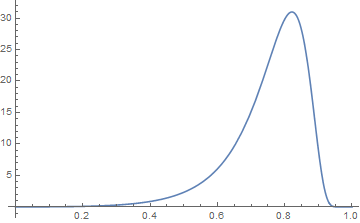
\includegraphics{graph2}
	\caption{Graph of the integrand after transformation of F(x)}
\end{figure}

By direct evaluation, $G(0)=G(1)=\infty$. But as the graph suggests, $\lim_{u \rightarrow 0^+} G(u) = \lim_{u \rightarrow 1^-} G(u) = 0$. For the purpose of numerical integration, it is reasonable to say that $G(0)=G(1)=0$.

Adaptive quadrature is now applicable on the bounded integral. The new integrand is quite complicated, but makes the limit of integration bounded.

\begin{equation}
I(x) = \int_{0}^{1} G(u)\;du
\end{equation}

The quadrature rules used for approximation are the trapezoid and Simpson's rules to gain optimal convergence rate. Rough estimate of the integral is set to 6. With these parameters, $\tilde{I}(x) = 6.493946262512657$, running time is 0.642 seconds with absolute error 6.860245828299583e-5.

\section{Results}
Lastly, a comparison among the numerical integration methods is necessary.

\begin{table}[H]
	\centering
	\begin{tabular}{c | c c c}
		Method & $\tilde{I}(x)$ & Runtime & Absolute Error \\
		\hline
		Simpson's $[0, 40]$ $h=0.001$ & 6.4939394022 & 0.266 s & 2.3270274596e-13 \\
		Adaptive $[0, 20]$ & 6.4939148767 & 0.397 s & 2.4525524218e-05 \\
		Gauss-Laguerre $n=8$ [0, 23] & 6.4939356653 & 0.279 s & 3.7369145422e-06 \\
		Transformed Adaptive [0,1] & 6.4939462625 & 0.642 s & 6.8602458282e-05
	\end{tabular}
\end{table}

Clearly, the Simpson's 2/3 rule performed the best among chosen numerical integration methods in terms of efficiency and accuracy. There are many factors that affect the performance of numerical integration methods, including the properties of integrand function, the limits of integration and properties of the transformed integrand function.

For the Gauss-Laguerre, one has to solve the nodal abscissas and weights, transform the integrand into some function and performing a finite sum. For the unbounded adaptive quadrature, a sufficient substitution must be employed first to transform the integrand into another function with bounded limits and then proceed with quadrature rule.

Remember that the performance of the methods mentioned above is due to a particular integrand function and its limits.

\section{Bibliography}
\begin{thebibliography}{9}
	\bibitem{bib:laguerre}
	Wolfram MathWorld, \emph{Gauss-Laguerre Quadrature}.
	\url{http://mathworld.wolfram.com/Laguerre-GaussQuadrature.html}
	
	\bibitem{bib:lagpoly}
	Wolfram MathWorld, \emph{Laguerre Polynomials}.
	\url{http://mathworld.wolfram.com/LaguerrePolynomial.html}
	
	\bibitem{bib:assoc}
	Wolfram MathWorld, \emph{Associated Laguerre Polynomials}.
	\url{http://mathworld.wolfram.com/AssociatedLaguerrePolynomial.html}
	
	\bibitem{bib:lagdiff}
	Wolfram MathWorld, \emph{Laguerre Differential Equation}.
	\url{http://mathworld.wolfram.com/LaguerreDifferentialEquation.html}
	
	\bibitem{bib:delta}
	Wolfram MathWorld, \emph{Kronecker Delta Function}.
	\url{http://mathworld.wolfram.com/KroneckerDelta.html}
	
	\bibitem{bib:delta}
	\emph{Improper Integrals}.
	\url{http://http://online.sfsu.edu/meredith/Numerical_Analysis/improper_integrals}
	
	\bibitem{bib:sci}
	Michael Health, \emph{Scientific Computing - An Introductory Survey}. Mc-Graw Hill. 2002
\end{thebibliography}

\end{document}